%!TEX root = JournalChapter1.tex
\section{Understanding microblog documents}
\label{discussion}

In this Section we first study the structure of microblog documents in order to define a hypotheses that captures their relevance. Subsequently, we test our hypotheses through the implementation of a number of approaches that capture microblogs' structure and their evaluation with respect to our DFR baseline. Additionally, we evaluate the relation of the order of the different dimensions within the microblogs, and determine how to utilise this evidence for ad-hoc retrieval.

\subsection{Informativeness of Microblogs}

For web and similar documents, relevance is modelled by the inclusion of statistical measures extracted both from the collection as a whole, and the documents themselves. Most retrieval models take into consideration document based statistics, such as document length and term frequency, in an attempt to capture the relevance of the documents according to the scope and verbosity hypotheses (or similar assumptions). For the purposes of this work, we can think of each retrieval model as a delicate relationship ``\(\circled{?}\)'' between document length \(|D|\) and term frequency \( P(q\, \cap\, D | Q)\) amongst other components. We pay attention to those components as they are most likely affected by the structure of microblogs.

\begin{equation}
 P(I|Q,D) = |D|\, \circled{?}\, P(q\, \cap\, D | Q)
  \vspace{0.5cm}
\end{equation}

Microblog documents are however very short as they have a fixed maximum size. Additionally, authors tend to optimise their content to fit within the character limits and constraints set by the platform, leading to a more or less constant document length ( \(\sim15\) terms in the case of Twitter). Moreover, due to these limitations, the value of term frequencies revolve around \(\sim1.5\). Thus in-document statistical information is limited.

Both the \textbf{scope} and \textbf{verbosity} hypotheses are defined within the assumption that authors may write as much as they desire. As a result it is logical to assume that when this condition is broken unexpected behaviour may follow. Fortunately, microblog documents contain other inherent features which encode extra information in the same message following an organic community-agreed vocabulary. In our work we draw inspiration from the ideas behind the scope and verbosity hypotheses and we are set to describe a new hypotheses tailored to microblog retrieval, which highlights and relies on characteristics of microblog documents' structure. 

Firstly, we assume that microblog documents (\textbf{D}) are 4-dimensional entities comprised of \textbf{Text \(T(D)\);} a \textbf{URL \(U(D)\)} ( Linking to an external resource); \textbf{Hashtags \(\#(D)\)} (Terms preceded by \#) indicating a topical context and \textbf{Mentions \(@(D)\)} (Terms preceded by @) indicating an intended audience. We believe that the amount of space in a microblog document dedicated to each of the dimensions may have a connection with how likely it is to be relevant to the searcher. Having these characteristics in mind, we define (\textbf{H1}) \textbf{Microblog Informativeness} (MI) as the probability for a Microblog document \(D\) being informative given a query \(P(MI|Q,D)\), which depends on an optimal unobserved combination ``\(\circled{?}\)'' of the aforementioned dimensions:

\begin{equation}
 P(MI|Q,D) =  T(D)~ \circled{?}~  U(D)~  \circled{?}~  \#(D)~  \circled{?}~  @(D) \circled{?}\, P(q\, \cap\, D | Q) %,
\end{equation} \\

\noindent where \(T(D)\), \(U(D)\), \(\#(D)\) and \(@(D)\) are the ratios in terms of number of characters spent in the document for each of the dimensions considered \footnote{URL's are automatically shortened by Twitter, thus their length is constant.}. For example, the ratio for the text dimension  \(T(D)\) is given by:

\begin{equation}
	T(D)= \frac{\# of Chars for Text Dimension}{ Total \# of Chars},
\end{equation}\\

In order to test our hypotheses and learn about what are the most prominent characteristics that make up relevant microblog documents, we analyse retrieval runs produced by the state of the art baseline DFR because it is the best performing model as shown in Table \ref{traditional}. We use the documents in the runs instead of all documents in the relevance judgements in order to analyse the documents that are most likely to contain query terms and find differences amongst those documents.

We take into consideration the TREC Microblog topics 1 to 110 so that we can confirm our findings through an evaluation on the newer 111 to 170 topics which belong to TREC's 2013 iteration of the microblog search task.



\begin{table*}[]
\begin{smaller}
\vspace{0.5cm}
\caption{Ratio of each dimension for relevant (Rel) and non-relevant (Non-Rel) documents at different cutoffs.}
\label{ratiosTable}
\vspace{0.30cm}
\begin{subtable}[b]{0.32\textwidth}
\caption{Cutoff @ 10}
\vspace{-0.5cm}
\begin{center}
\begin{tabular}{|c|c|c|}

\hline  & Rel & Non-Rel \\ 
\hline Hash & 1.960 &  	1.619  \\
\hline Ment & 2.750 &  	2.444  \\
\hline Urls & 17.32 &  	14.16 * \\
\hline Text & 77.95 &  	81.77 * \\ 
\hline
\hline DocLength & 97.47 &  	100.2  \\
\hline 
\end{tabular} 
\end{center}
\label{ratio10}
\end{subtable}
~
\begin{subtable}[b]{0.32\textwidth}
\caption{Cutoff @ 20}\vspace{-0.5cm}
\begin{center}
\begin{tabular}{|c|c|c|}


\hline  & Rel & Non-Rel \\ 
\hline Hash & 2.626 &  	1.861 * \\
\hline Ment & 2.453 &  	2.402  \\
\hline Urls & 17.54 &  	13.54 * \\
\hline Text & 77.37 &  	82.18 * \\
\hline
\hline DocLength & 96.50 &  	97.38  \\
\hline 
\end{tabular} 
\end{center}
\label{ratio20}
\end{subtable}
~
\begin{subtable}[b]{0.32\textwidth}
\caption{Cutoff @ 30}\vspace{-0.5cm}
\begin{center}
\begin{tabular}{|c|c|c|}
\hline  & Rel & Non-Rel \\ 
\hline Hash & 2.514 &  	1.999  \\
\hline Ment & 3.061 &  	2.671  \\
\hline Urls & 17.13 &  	14.28 * \\
\hline Text & 77.29 &  	81.04 * \\
\hline
\hline DocLength & 96.21 &  	95.76  \\
\hline 
\end{tabular} 
\end{center}
\label{ratio30}
\end{subtable}

\hspace{1.8cm}
\begin{subtable}[]{0.35\textwidth}

\caption{Cutoff @ 50}\vspace{-0.45cm}
\begin{center}
\begin{tabular}{|c|c|c|}

\hline  & Rel & Non-Rel \\ 
\hline Hash & 2.820 &  	2.518  \\
\hline Ment & 2.968 &  	3.136  \\
\hline Urls & 17.19 &  	14.32 * \\
\hline Text & 77.01 &  	80.01 * \\
\hline
\hline DocLength & 95.90 &  	94.45  \\
\hline 
\end{tabular} 
\end{center}
\label{ratio50}
\end{subtable}
~
\begin{subtable}[]{0.35\textwidth}
\caption{Cutoff @ 100}\vspace{-0.45cm}
\begin{center}
\begin{tabular}{|c|c|c|}
\hline  & Rel & Non-Rel \\ 
\hline Hash & 2.638 &  	2.514  \\
\hline Ment & 2.893 &  	3.315 * \\
\hline Urls & 17.69 &  	14.13 * \\
\hline Text & 76.77 &  	80.03 * \\
\hline
\hline DocLength & 93.96 & 92.56  \\
\hline 
\end{tabular} 
\end{center}
\label{ratio100}
\end{subtable}


\end{smaller}
\vspace{0.70cm}
\end{table*}







Tables \ref{ratiosTable}(a...e) introduce the mean ratios for each of the dimensions for all documents at the cut-offs @10, @20, @30, @50 and @100 respectively. The asterisk indicates statistically significant differences between relevant and non-relevant documents for that dimension. The last row on each table on the other hand, indicates the average document length in number of characters for both relevant and non-relevant documents.

First we look at ``DocLength''. As we can observe in Tables \ref{ratiosTable}(a...e), the differences between relevant and non-relevant documents are not significant. Furthermore, we can see how relevant documents tend to be shorter than non-relevant documents for cut-offs @10 and @20, whereas then they become longer than non-relevant documents for any cut-off after @20. It is evident that the behaviour of this feature is unstable, and the differences between both groups of documents change wildly depending on the cut-off point, contradicting each other.

Based on this observation we can conclude that the document length feature, popular amongst retrieval models, is ineffective in estimating the relevance of a microblog document. Therefore, this helps us to confirm that the scope and verbosity hypothesis do not hold for microblog documents, as differences should have followed a more clear trend if the hypotheses were true. (i.e. One relevance group should have remained higher than the other for all cut-off cases.). Therefore we can confirm that in the case of microblog documents, longer (or shorter) does not have a connection with a document being relevant. 

Secondly, we look at the \textbf{Urls} and \textbf{Text} dimensions of microblog documents in Figure \ref{urltext}. In the case of \textbf{Urls}, this dimension tends to be significantly larger on relevant documents than in their non-relevant counterparts. This is in line with previous works suggesting that the presence of URL's increases the likelihood for a document to be relevant \cite{massoudi2011incorporating}. Figure \ref{Urls} shows the changes in space dedicated to the URL dimension as we go down the results list. An interesting behaviour that can be observed is that, relevant documents behave in exactly the opposite way to non-relevant documents. As we traverse the results list the space for the URL's in relevant documents increases whereas, it slowly decreases for non-relevant documents.

The \textbf{Text} dimension on the other hand, is significantly smaller for relevant documents, across all cut-offs. However, as observed in Figure \ref{Text}, the behaviour as we traverse the list towards lower cut-off points is similar for both relevant and non-relevant documents. Thus the differences in characters dedicated to this dimension remain stable between relevant and non-relevant documents.

The stability in the differences of both the \textbf{Urls} and \textbf{Text} dimensions make them especially interesting feature candidates to be studied, and possibly employed to improve the behaviour of retrieval systems.

%!TEX root = main.tex



\begin{figure*}
\begin{smaller}
    \centering
       \hspace{-0.5cm}
        \begin{subfigure}[b]{0.4\textwidth}
        	        \centering
                    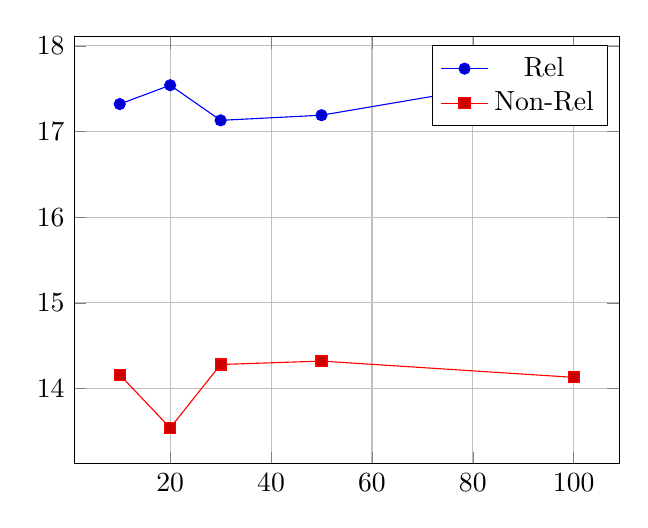
\begin{tikzpicture}
        	\begin{axis}[
        		height=7cm,
        		width=8.5cm,
        		grid=major,
        	]
        	\addplot coordinates {
        		(10,17.32)
        		(20,17.54)
        		(30,17.13)
        		(50,17.19)
        		(100,17.69)
        	};
        	\addlegendentry{Rel}
        			
        	\addplot coordinates {
        		(10,	14.16)
        		(20,	13.54)
        		(30,	14.28)
        		(50,	14.32)
        		(100,	14.13)
        		
        	};
        	\addlegendentry{Non-Rel}
        
        
        	\end{axis}
        	
        \end{tikzpicture}
        \caption{Urls}
        \label{Urls}
        \end{subfigure}
		~
		\hspace{1.5cm}
        \begin{subfigure}[b]{0.4\textwidth}
        	        \centering
                    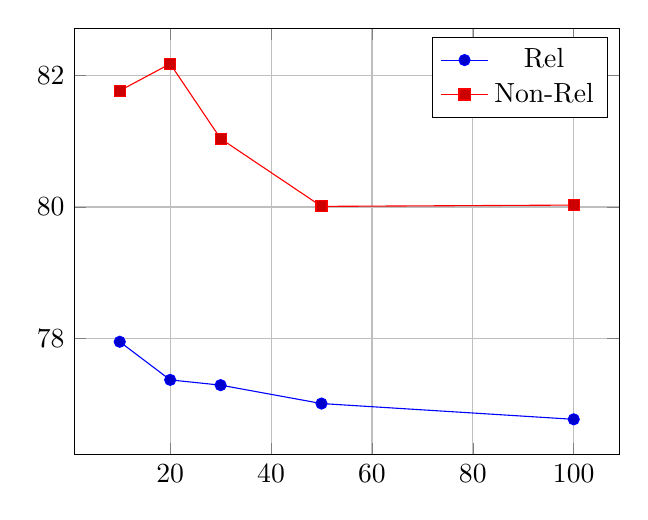
\begin{tikzpicture}
        	\begin{axis}[
        		height=7cm,
        		width=8.5cm,
        		grid=major,
        	]
        	\addplot coordinates {
        	(10,77.95)
        	(20,77.37)
        	(30,77.29)
        	(50,77.01)
        	(100,76.77)
        	};
        	\addlegendentry{Rel}
        			
        	\addplot coordinates {
        		(10,	81.77)
        		(20,	82.18)
        		(30,	81.04)
        		(50,	80.01)
        		(100,	80.03)
        	};
        	\addlegendentry{Non-Rel}
        
        
        	\end{axis}
        	
        \end{tikzpicture}
        \caption{Text}
        \label{Text}
        \end{subfigure}
\end{smaller}
\caption{Rate (\%) of space dedicated to Urls and Text in Relevant and Non-Relevant documents at different cut-off points.}
\label{urltext}
\vspace{0.5cm}
\end{figure*}








Figure \ref{hashtagMention} shows the behaviour for the Hash and Mention dimensions. In terms of the \textbf{Hash} dimension, differences are only significant when looking at the @20 cut-off. Additionally, relevant documents seem to have a higher portion of the content dedicated to this dimension than non-relevant documents. This behaviour can be observed in Figure \ref{Hashtags}, as relevant documents seem to dedicate more space for hashtags regardless of the cut-off chosen. Another observation that can be made, is that as we traverse the result list, the presence of hashtags become more pronounced for both relevant and non-relevant documents, thus the increased (or decreased) presence of hashtags does not serve as a discriminative factor in microblog ranking.

Finally, we observe the behaviour of the \textbf{Mention} dimension in Figure \ref{Mentions}. For the three first cut-offs @10; @20 and @30, relevant documents seem to spend more space in defining an audience than non-relevant documents. After the @30 cut-off the roles are swapped and non-relevant documents spend more space in referring to the target users than relevant documents. This makes sense if we assume that many non-relevant documents may be conversational in nature, instead of introducing facts interesting to a wider audience. In fact the differences in terms of the space dedicated to the \textbf{Mentions} dimension is only significant once we are much lower in the ranking at the @100 cut-off.

One could argue that our conclusions may be biased since the result lists are produced with respect to the retrieval model inherent features (e.g. document length). However, we can see that the differences in the observations between relevant and non-relevant documents for the good dimensions (Urls, Text and Hash) are relatively constant, thus independent from the rank for our purposes.

\subsection{Modelling Microblog Informativeness}
In the previous section we observed that relevant Microblog documents present different characteristics to those non-relevant in terms of the aforementioned dimensions (Figure \ref{dimensionaltweet}). More specifically, relevant documents tend to use less space for text, and more space to contain the URLs, and hashtag dimensions than non-relevant documents. An important note is that we cannot assume that the less space dedicated to text the more relevant the document will be, as that would make a text-less document the one with the highest likelihood of being relevant. 

Therefore, we estimate that a relevant document has an optimal amount of space dedicated to the text dimension which ranges from 76\% to 78\% as observed in Figure \ref{Text}. Thus we model informativeness in terms of the retrieval model score \(P(q \cap D|Q)\) for document \(D\) given query \(Q\) and its Text dimension as: 

\begin{figure}[]
	\centering
	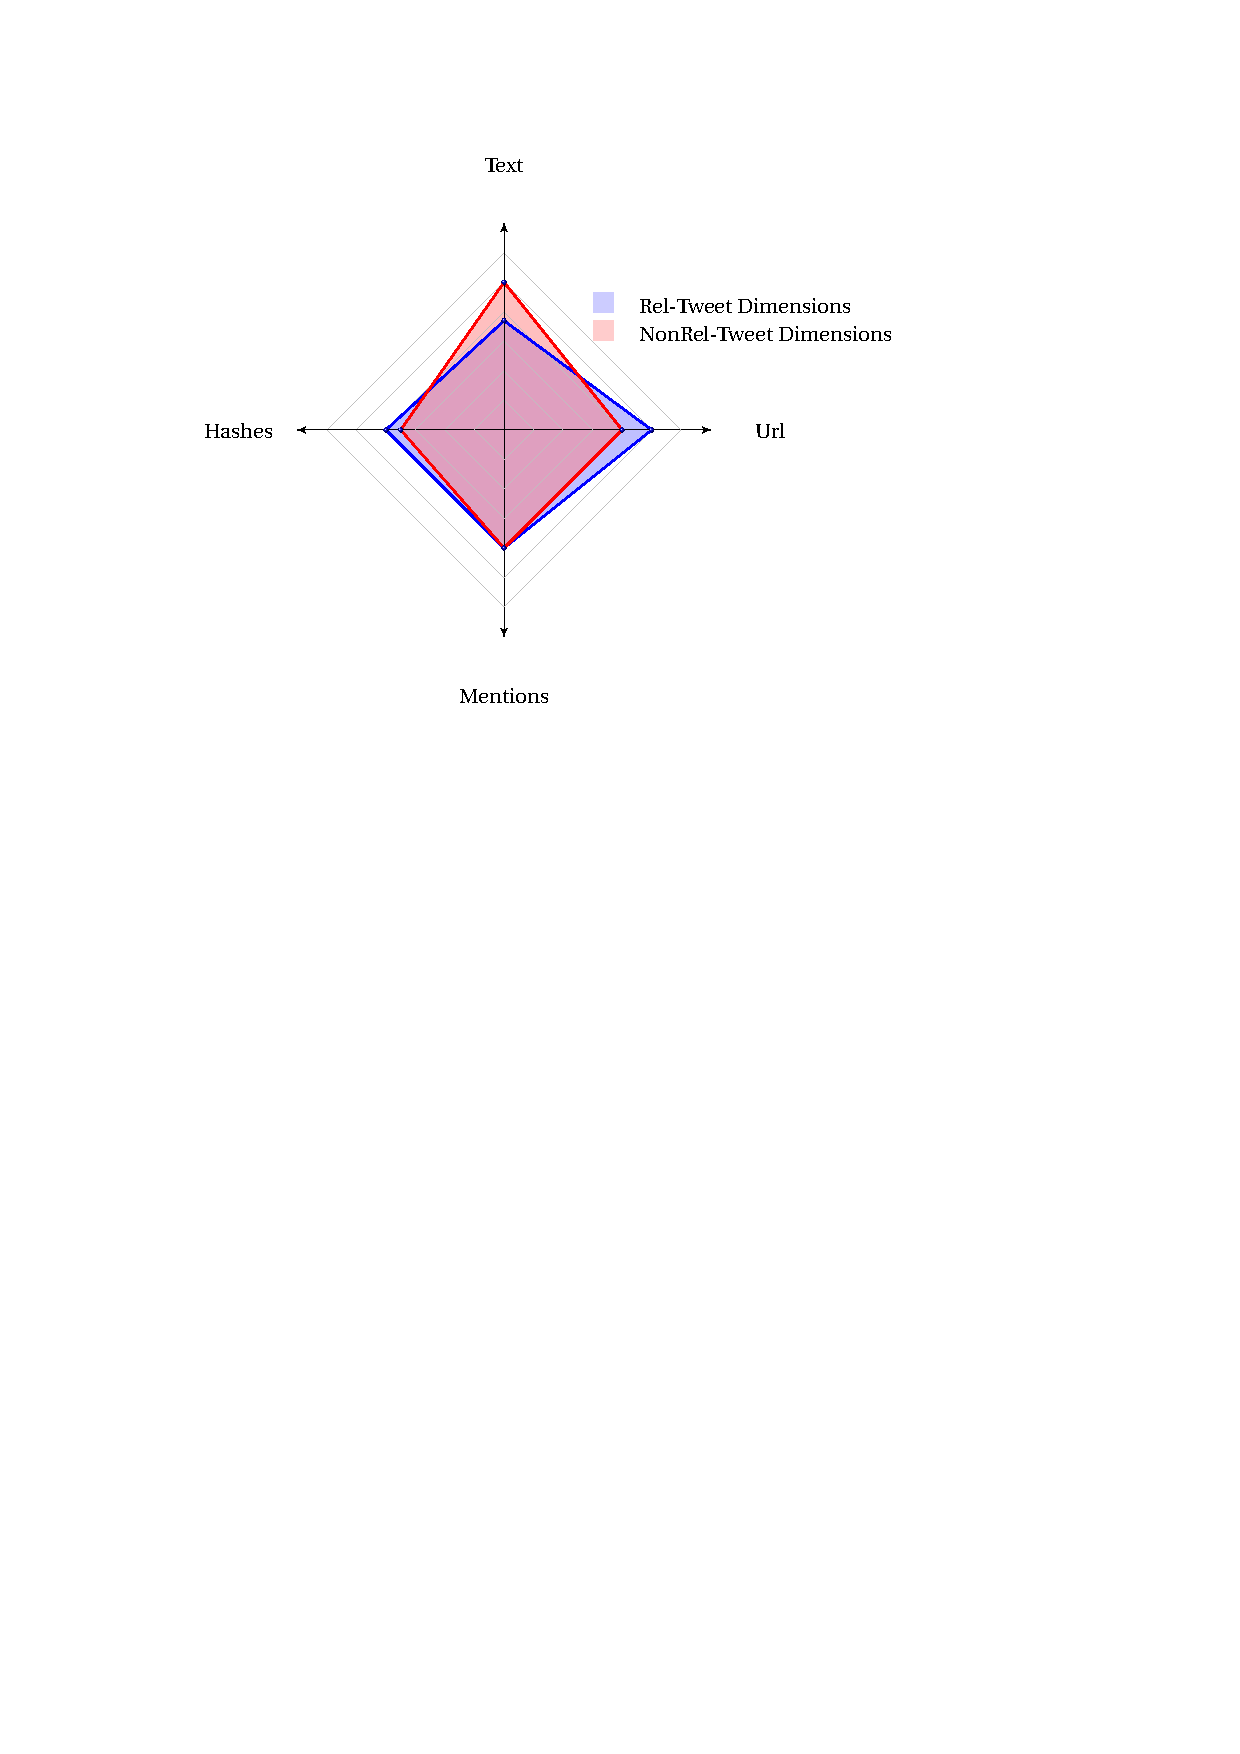
\includegraphics[trim = 30mm 175mm 58mm 22mm, clip, width=11.5cm]{kiviat.pdf}
	\caption{Dimensional differences between relevant and non-relevant documents. Statistically significant differences are exaggerated for easier visualization.}
	\label{dimensionaltweet}
\end{figure}

\begin{equation}
P(MI|D,Q) = P(q \cap D|Q) + \lambda [1- \abs{T(D)-0.76}],
\label{eqText}
\end{equation}\\

\noindent where we give a lower score to those documents diverging from the optimal text dimension rate 0.76\footnote{The optimal 76\% rate of presence for the text dimension specified above, which we normalise between 0 and 1.}. We test this formulation using DFR to produce the \(P(q \cap D|Q)\) score over the microblog 2013 collection, which was \textbf{not} used in producing the analysis results in the previous section. We retrieve the first 500 documents using DFR and re-rank them using our first model (Equation \ref{eqText}) with \(\lambda\) set to 1. The results are shown in the RR-text\footnote{``RR-'' stands for ``Re Ranking'', and precedes the features utilised in the operation} row within Table \ref{dimResults}. As we can observe, the performance of DFR is enhanced by taking into account the textual dimension of the microblog documents, being statistically significantly better in terms of P@20.

\begin{figure}

\begin{smaller}
        \begin{subfigure}[b]{0.2\textwidth}
	        \centering
               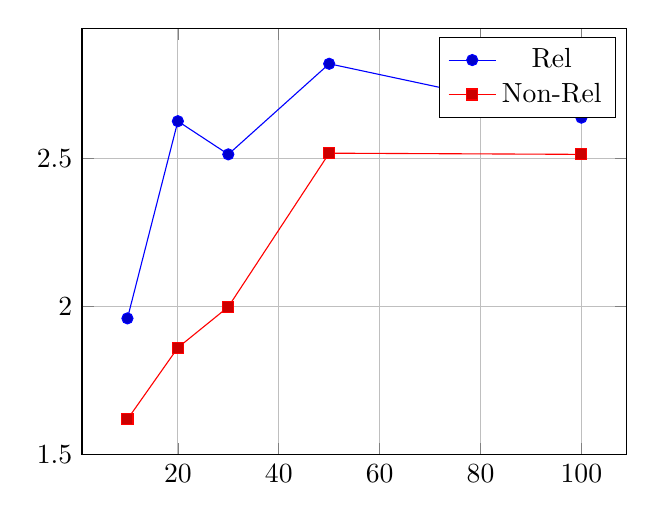
\begin{tikzpicture}
               	\begin{axis}[
               		height=7cm,
               		width=8.5cm,
               		grid=major,
               	]
               	\addplot coordinates {
              		(10.0,1.96)
               		(20.0,2.626)
               		(30.0,2.514)
               		(50.0,2.82)
               		(100.0,2.638)
               	};
               	\addlegendentry{Rel}           			
               	\addplot coordinates {
               		(10.0,	1.619)
               		(20.0,	1.861)
               		(30.0,	1.999)
               		(50.0,	2.518)
               		(100.0,	2.514)
               	};
               	\addlegendentry{Non-Rel}
               \end{axis}       	
               \end{tikzpicture}
               \caption{Hashtags}

               \label{Hashtags}

        \end{subfigure}%
        ~
        \hspace{4.5cm}
        \begin{subfigure}[b]{0.2\textwidth}
	        \centering
            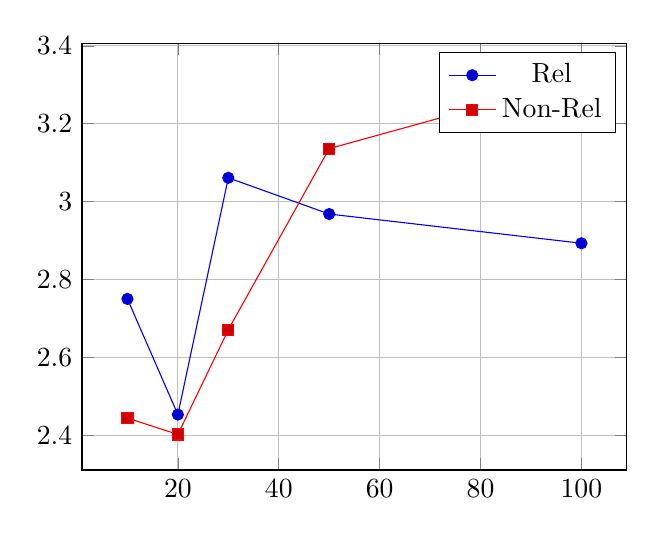
\begin{tikzpicture}
        	\begin{axis}[
        		height=7cm,
        		width=8.5cm,
        		grid=major,
        	]
        	\addplot coordinates {
        		(10,2.75)
        		(20,2.453)
        		(30,3.061)
        		(50,2.968)
        		(100,2.893)
        	};

        	\addlegendentry{Rel}
        	\addplot coordinates {
        		(10,	2.444)
        		(20,	2.402)
        		(30,	2.671)
        		(50,	3.136)
        		(100,	3.315)
        	};
        	\addlegendentry{Non-Rel}
        	\end{axis}
        \end{tikzpicture}
        \caption{Mentions}
        \label{Mentions}
        \end{subfigure}

\end{smaller}

\caption{Rate (\%) of space dedicated to HashTags and Mentions in Relevant and Non-Relevant documents at different cut-off points.}
\label{hashtagMention}

\end{figure}

Similarly, we combine the URL dimension expressed as a rate with the score of the retrieval model as follows:

\begin{equation}
P(MI|D,Q) = P(q \cap D|Q) + \omega U(D),
\label{eqUrl}
\end{equation}\\

\noindent where we set the free parameter \(\omega\) to 1. The results obtained for the experiments with this model are shown in Table \ref{dimResults} in row RR-Url. The use of the URL dimension on its own also improves the performance over the DFR itself, most significantly for P@10 and P@20. Furthermore, it produces slightly better results than the RR-Text approach. Additionally we combined both models to produce: 

\begin{equation}
P(MI|D,Q) = P(q \cap D|Q) + \lambda [1- \abs{T(D)-0.76}] + \omega U(D),
\label{eqComb}
\end{equation}\\

The results for this combination are shown in Table \ref{dimResults} as row RR-text-url. Further improvements with respect to previous approaches are introduced at all cut-offs except P@10, where RR-url performs slightly better than the combined approach. Finally we also added components to account for the hash and mention dimensions, producing the following two models:

\begin{equation}
\begin{split}
P(MI|D,Q) = P(q \cap D|Q) + \lambda [1- \abs{T(D)-0.76}] \\
 + \omega U(D) + \gamma \#(D),
\end{split}
\label{eqHash}
\end{equation}\\

\begin{equation}
\begin{split}
P(MI|D,Q) = P(q \cap D|Q) + \lambda [1- \abs{T(D)-0.76}] \\
 + \omega U(D) + \gamma \#(D) + \delta @(D),
\end{split}
\label{eqMent}
\end{equation}\\

\noindent where the free parameters are set to 1\footnote{Parameter optimisation would be beneficial in the future, although it was not necessary to evaluate the hypothese of this work}.

The results for both models (Equations \ref{eqHash} and \ref{eqMent}) are shown in Table \ref{dimResults} as RR-text-url-hash and RR-text-url-hash-ment respectively. The performance achieved by adding the hash component over the previous models is further increased specially for P@10, whereas it performs slightly worse than RR-text-url in terms of P@30. The addition of the mentions component in RR-text-url-hash-ment reduces retrieval performance across P@10, P@15 and P@20 with respect to the last model.

If we consider Figures \ref{Urls}, \ref{Text}, \ref{Hashtags} and \ref{Mentions} and Table \ref{dimResults} we can see how the dimensions that showed constant differences across all cut-offs are the features enhancing the performance of the baseline. The only feature which results in poorer retrieval performance is the mentions dimension, which as observed in Figure\ref{Mentions} follows an erratic behaviour (For earlier cut-offs more space is dedicated to the mentions in relevant documents, and then after the cut-off 40 is the opposite case).

\begin{table}[]
\caption{Experimental results when considering different dimensions, using the 2013 TREC Microblog collection (*\(p <0.05 \) over the DFR baseline).}
\centering
\begin{tabular}{|c|c|c|c|c|c|}
\hline Model & P@5 & P@10  & P@15  & P@20  & P@30  \\
\hline
DFR & 0.65 & 0.59 & 0.54 & 0.51 & 0.45 \\
\hline
text & 0.65 & 0.59 & 0.54 & 0.52* & 0.45 \\
url & 0.65 & 0.61* & 0.54 & 0.52* & 0.46 \\
text-url & 0.66* & 0.61* & 0.55* & 0.52* & \textbf{0.47} \\
text-url-hash & \textbf{0.66*} & \textbf{0.62*} & \textbf{0.56*} & \textbf{0.53*} & 0.46 \\
text-url-hash-ment & 0.66* & 0.61* & 0.55 & 0.52* & 0.46 \\
\hline 
\end{tabular} 
\label{dimResults}
\vspace{0.30cm}
\end{table}

Based on our experimental results, we can assert that there are structural differences between relevant and non-relevant documents in terms of the dimensions defined in this work. More specifically, we have come up with a possible instantiation which captures Microblog characteristics in the shape of a model given by Equation \ref{eqHash}. The implications of these findings and experiments are that users produce Microblog documents in different ways, with certain formats more likely to satisfy the information need of a searcher. In the following subsection, we expand our analysis by taking into consideration the order of the dimensions.